% Global document settings
\documentclass[10pt]{article}

% Packages
\usepackage{tgtermes}
\usepackage{graphicx}
\usepackage{natbib}
\usepackage{authblk}
\usepackage{array}
\usepackage{colortbl}
\usepackage{tocloft}
\usepackage{xcolor}
\usepackage{siunitx}
\usepackage{setspace}
\usepackage{listings}
\usepackage{caption}
\usepackage[T1]{fontenc}
\usepackage[nottoc]{tocbibind}
\usepackage[breaklinks]{hyperref}
\usepackage[font=small,skip=7pt]{caption}

% Custom colours
\definecolor{codegreen}{rgb}{0,0.6,0}
\definecolor{codegray}{rgb}{0.5,0.5,0.5}
\definecolor{codepurple}{rgb}{0.58,0,0.82}
\definecolor{backcolour}{rgb}{0.95,0.95,0.92}

% Listing styles
\lstdefinestyle{mystyle}{
  backgroundcolor=\color{backcolour},
  commentstyle=\color{codegreen},
  keywordstyle=\color{purple},
  numberstyle=\tiny\color{codegray},
  stringstyle=\color{codepurple},
  basicstyle=\ttfamily\footnotesize,
  breakatwhitespace=false,
  breaklines=true,
  captionpos=b,
  keepspaces=true,
  numbers=left,
  numbersep=5pt,
  showspaces=false,
  showstringspaces=true,
  showtabs=false,
  tabsize=2
  }
  \lstset{style=mystyle}

  % Custom commands
  \renewcommand{\bibname}{References} % Change bibliography title
  \renewcommand\cftsecafterpnum{\vskip8pt}
  \renewcommand{\lstlistlistingname}{List of \lstlistingname s}
  \renewcommand{\bibsection}{\section*{Bibliography}}
  \renewcommand{\contentsname}{Table of Contents}
  \renewcommand{\bibsection}{\section{\bibname}}
  \renewcommand{\cftsecleader}{\cftdotfill{\cftdotsep}}

  % Custom settings
  \captionsetup{justification=centering}
  \PassOptionsToPackage{hyphens}{url}
  \urlstyle{same}
  \def\Urlmuskip{0mu}
  \def\UrlBreaks{\do\/\do-}
  \hypersetup{
    colorlinks = true,
    urlcolor = blue,
    linkcolor = black,
    citecolor = black,
  breaklinks=true,
  pdfpagemode=UseOutlines,
  bookmarksopen=true,
  bookmarksopenlevel=2,
  bookmarksnumbered=true
  }

  \title{\textbf{Flicking the Switch: } \\ Optogenetics and the Interplay of Direct and \\ Indirect Pathways in Motor Control}
  % \author[ ]{Daniel Burger}
  \author[ ]{K23003985}
  \affil[ ]{\textbf{King’s College London}}
  \affil[ ]{\href{mailto:K23003985@kcl.ac.uk}{K23003985@kcl.ac.uk}}
  \date{\textit{8. August 2023}}

\begin{document}
\pagenumbering{roman}
\counterwithin{lstlisting}{section}
\counterwithin{figure}{section}
\counterwithin{table}{section}

\maketitle
\thispagestyle{empty}

% Double spacing for feedback
\doublespacing

\begin{sloppypar} % For better line breaks
  \begin{abstract}
    This essay presents a comprehensive synthesis of the current understanding of basal ganglia pathways, focusing on direct and indirect neural circuits. It critically evaluates the traditional dichotomous model and examines recent evidence suggesting a nuanced, dynamic interaction between the two pathways in motor control, decision-making, reward processing, and motor learning. Utilising key studies employing optogenetic techniques, the essay contributes to a deeper understanding of these pathways’ concurrent activation and divergence during action initiation and execution.

    Moreover, the essay delves into the implications of alterations in these pathways for the manifestation of Parkinson’s disease symptoms and potential therapeutic strategies for mitigating these symptoms. It also outlines the significant contributions of optogenetics to our knowledge of these pathways, underscoring the technique’s power and precision. Despite significant advancements in understanding basal ganglia circuit dynamics, the essay highlights open questions regarding the precise mechanisms coordinating pathway interactions during action selection and learning, underlining the need for continued research.
  \end{abstract}
  \pagebreak

  % \pagenumbering{Roman}
  % \tableofcontents
  % \pagebreak

  % \listoffigures
  % \pagebreak

  % \listoftables
  % \pagebreak

  % Back to normal numbering
  \pagenumbering{arabic}

  \section{Introduction}
  \label{sec:introduction}

  Parkinson’s disease, a prevalent neurodegenerative disorder, prominently manifests through motor symptoms. These include rigidity, which refers to stiffness and resistance to limb movement; tremors, involuntary, rhythmic and oscillating movements of a part of the body; and bradykinesia, which describes the slowness of movement and difficulty initiating movement seen in Parkinson’s patients. These symptoms are primarily attributed to the degeneration of dopaminergic neurons in the basal ganglia, a subcortical nucleus pivotal for motor control and decision-making \citep{kravitz_regulation_2010}. The conventional model of basal ganglia function posits two antagonistic pathways: the direct pathway, promoting movement, and the indirect pathway, inhibiting movement. Alterations in the balance and function of these pathways are thought to contribute to the motor deficits seen in Parkinson’s disease. However, this binary model has been challenged by recent evidence, suggesting a more nuanced interaction between these pathways with potential concurrent activation and divergence \citep{dunovan_believer-skeptic_2016}.

  The advent of optogenetic techniques, which allow for the precise manipulation of specific neurons using light, has significantly advanced our understanding of basal ganglia pathways \citep{kravitz_regulation_2010, cui_concurrent_2013}. Studies by \cite{kravitz_regulation_2010} provided evidence for certain aspects of the traditional model through optogenetic activation of direct and indirect pathway medium spiny neurons (MSNs). This pioneering work paved the way for other optogenetic investigations that have further expanded our comprehension of the complexity of these pathways, suggesting they may function bidirectionally \citep{yttri_opponent_2016} to regulate motor behaviour through selective stimulation.

  More recently, studies such as those by \cite{hilt_evidence_2016} and \cite{wang_direct_2015} have further expanded our understanding of the role of these pathways in reward-based learning, motor learning, and the regulation of movement velocity.

  Armed with this context, this essay aims to synthesise the current knowledge and debates surrounding the role of basal ganglia pathways in motor control and decision-making, focusing on the insights provided by optogenetic studies.

  \section{Overview and Findings of Cui et al. (2013) Study}
  \label{sec:cui-et-al-2013}

  The study by \cite{cui_concurrent_2013} marked a significant step forward in understanding basal ganglia pathways. The researchers contested the traditional model, which posits the direct and indirect pathways of the basal ganglia as independent entities. They suggested a more dynamic interaction between them during action selection.

  To investigate this, \cite{cui_concurrent_2013} utilised optogenetic techniques, a ground-breaking method that allows the manipulation of specific neurons using light, providing precise control over neuronal activity. Their focus was on the medium spiny neurons (MSNs) located in the dorsomedial striatum of mice, which form the origin points of the direct and indirect pathways.

  The most significant revelation from \cite{cui_concurrent_2013}’s study was the concurrent activation of the direct and indirect pathways during action initiation as shown in \autoref{fig:pathway-activation}. They found that both direct-pathway MSNs (dMSNs) and indirect-pathway MSNs (iMSNs) increased their firing rates before initiating a movement, which counters the classical model’s assertion of opposing activation of these pathways.

  \begin{figure}[ht]
    \centering
    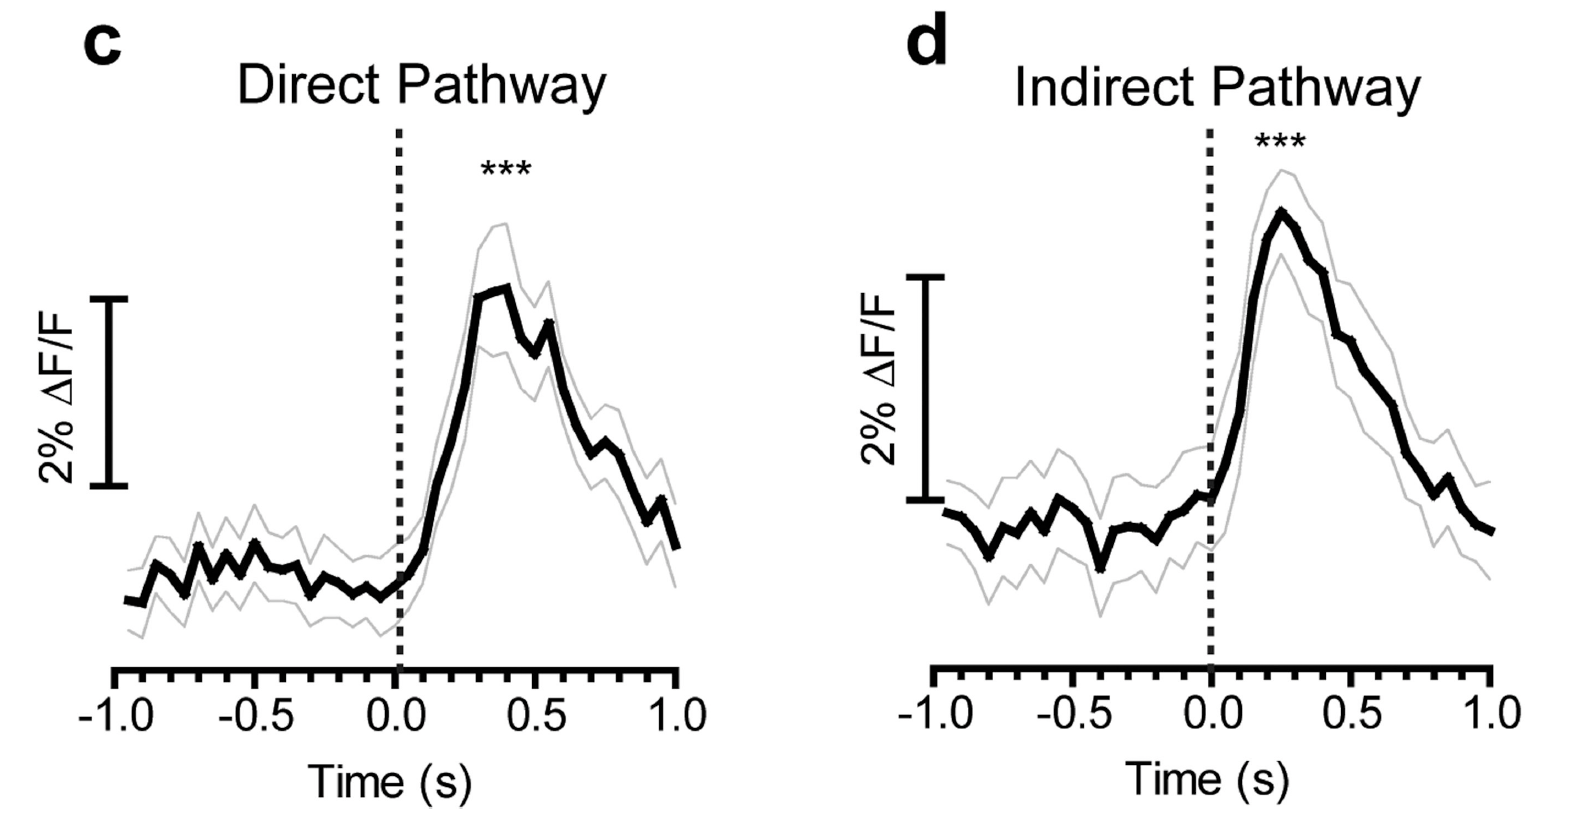
\includegraphics[width=\textwidth]{figures/direct-indirect-activation.png}
    \caption[Concurrent activation of direct and indirect pathways during action initiation]{\textbf{Concurrent activation of direct and indirect pathways during action initiation.} This figure presents data from \cite{cui_concurrent_2013}’s study, specifically parts c and d of their original Figure 2, demonstrating the concurrent activation of direct-pathway medium spiny neurons (dMSNs) and indirect-pathway medium spiny neurons (iMSNs) at the start of a lever-pressing session. The fluorescence traces indicate increased activity for both dMSNs and iMSNs at the session start, countering the classical model’s assertion of opposing activation of these pathways. This suggests a more complex interplay between the direct and indirect pathways during action initiation, challenging traditional models of basal ganglia function.}
    \label{fig:pathway-activation}
  \end{figure}

  Interestingly, they observed a decrease in the activity of iMSNs during movement, a change not seen in dMSNs. This finding indicates that while both pathways are involved in action initiation, their roles may diverge during action execution. Additionally, \cite{cui_concurrent_2013} found that both dMSNs and iMSNs were quiet during inactive states when the mice were not moving, further challenging the traditional model.

  These findings were further supported by a study by \cite{guillaumin_experimental_2021}, which explored the role of the direct and indirect pathways in reward-based learning. The researchers found that activating the direct pathway enhanced reward-seeking behaviour while activating the indirect pathway suppressed it. This lends further credence to the complex, dynamic interaction between the direct and indirect pathways in the basal ganglia.

  \section{Optogenetics in Decoding Neural Pathways}
  \label{sec:the-role-of-optogenetics-in-neural-pathways}

  Optogenetics, a revolutionary tool in neuroscience, employs light-sensitive proteins known as opsins to control and observe specific neurons’ activity in living tissue. This technique, offering unprecedented precision, has greatly enhanced our understanding of the basal ganglia pathways.

  It was \cite{kravitz_regulation_2010} who first employed optogenetics to selectively activate striatal medium spiny neurons (MSNs) in mice, the cell types that form the direct and indirect pathways. Their pioneering work paved the way for other optogenetic investigations into basal ganglia pathways.

  Later, \cite{cui_concurrent_2013} utilised optogenetic techniques to measure the activity of direct and indirect pathway MSNs in mice during movement initiation. Their findings challenge the traditional model by showing increased activity in both pathways prior to movement initiation.

  More recently, researchers have continued to harness the power of optogenetics to further our understanding of the basal ganglia’s direct and indirect pathways. For example, \cite{yttri_opponent_2016} used cell-type-specific optogenetic stimulation to investigate the bidirectional control of movement velocity.

  However, it is crucial to acknowledge the limitations of optogenetics. The need for genetic modifications can pose challenges in certain settings, and delivering light to deep brain structures can be technically challenging. Despite these limitations, optogenetics has greatly enhanced our understanding of neural circuits and holds promise for future studies and potential therapeutic applications.

  In conclusion, optogenetics has emerged as a powerful tool in neuroscience, providing novel insights into the functioning of neural pathways, including the direct and indirect pathways of the basal ganglia. As our understanding and application of optogenetics continue to evolve, we expect it to shed more light on the brain’s complex workings.

  \section{Complementary and Contrasting Studies}
  \label{sec:complementary-and-contrasting-studies}

  Beyond the work of \cite{cui_concurrent_2013} and \cite{kravitz_regulation_2010}, several other studies have significantly contributed to our understanding of the direct and indirect pathways in the basal ganglia.

  \cite{yttri_opponent_2016} further explored these pathways’ roles in the bidirectional control of movement velocity using optogenetic stimulation. Their findings provided evidence that both pathways can bidirectionally regulate movement velocity and speed, complementing \cite{cui_concurrent_2013}’s finding of concurrent activation during action initiation.

  In a different vein, \cite{guillaumin_experimental_2021} investigated the role of these pathways in reward-based learning. They found that activating the direct pathway enhanced reward-seeking behaviour while activating the indirect pathway suppressed it. These findings demonstrate the involvement of both pathways in reward processing, which differs from \cite{cui_concurrent_2013}’s observations about movement initiation.

  \cite{hilt_evidence_2016} turned their focus to motor learning. They found that activating the direct pathway facilitated motor learning, while activating the indirect pathway impaired it. This highlights the dynamic interplay between these pathways in motor skill acquisition.

  Lastly, \cite{wang_direct_2015} explored how these pathways regulate movement speed control. They found that the direct pathway increased speed while the indirect pathway decreased it. These findings provide evidence for the opposing roles of these pathways in velocity and speed regulation.

  \section{Conclusion}
  \label{sec:conclusion}

  Collectively, these studies emphasise the multifaceted involvement of the direct and indirect pathways in various functions like reward processing, motor learning, and precise motor control. They demonstrate the utility of optogenetics in elucidating the nuanced interactions between these pathways.

  Our understanding of the basal ganglia’s direct and indirect pathways, including their diverse roles in motor control, decision-making, reward processing, and motor learning, has advanced significantly in recent years. While earlier models viewed these pathways in strict dichotomous terms, recent research highlights a more dynamic, nuanced interaction between them.

  However, open questions remain regarding the precise mechanisms coordinating pathway interactions during action selection and learning. As optogenetic techniques continue to be refined, future research can build on these discoveries to further elucidate the complexities of basal ganglia circuit dynamics and functions. Such advancements will have profound implications for understanding diseases involving basal ganglia dysfunction.

  In conclusion, while early models painted a binary picture of direct and indirect pathway opposition, contemporary evidence points to a more collaborative, context-dependent interaction between these pathways in functions like motor control and learning. Continued research into these complex neural circuits promises exciting breakthroughs in comprehending the basal ganglia’s multifaceted roles and neurologic disease.

  \pagebreak
  \singlespacing % No need for double spacing in the references
  \bibliographystyle{references/custom-apa}
  \bibliography{references/bibliography}

\end{sloppypar}
\end{document}